% begin{figure}[htbp] - 
%[h]ere, [t]op of the page, [b]ottom of the current page or [p]age for itself

% Fußnote in der Caption einer Figure: https://tex.stackexchange.com/a/67030
%  \caption[Caption for LOF]{Real caption\protect\footnotemark}
% \end{figure}
% \footnotetext{footnote text}

% Two tables next to each other https://tex.stackexchange.com/a/79616


% Laden eines TTT boards und Text daneben einfuegen - den State kann ich einfach noch inder Caption benennen
\begin{figure}
   \begin{minipage}[c]{.5\textwidth}
   \centering
    \includegraphics[]{05_Artefakte/01_Abbildungen/ttt_boards/ttt_figures.pdf}
   \end{minipage}%
   \begin{minipage}[c]{.5\textwidth}
      Some text describing the image.
      Some text describing the image.
      Some text describing the image.
   \end{minipage}
   \caption{Your image}
\end{figure}

% 4 Bilder als 2x2 Matrix 
% Alternativ auch diese Lösung: https://tex.stackexchange.com/a/357176/220502
\begin{figure}
    \centering
    \begin{subfigure}[b]{0.45\textwidth}
      \centering
      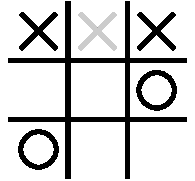
\includegraphics[scale=0.7]{ttt_boards/ttt_win.pdf}
      \caption{Win}
      \label{fig:ttt_win}
    \end{subfigure}
    \begin{subfigure}[b]{0.45\textwidth}
      \centering
      
\includegraphics[scale=0.7]{ttt_boards/ttt_block.pdf}
      \caption{Block}
      \label{fig:ttt_block}
    \end{subfigure}
    \begin{subfigure}[b]{0.45\textwidth}
      \centering
      
\includegraphics[scale=0.7]{ttt_boards/ttt_fork.pdf}
      \caption{Fork}
      \label{fig:ttt_fork}
    \end{subfigure}
    \begin{subfigure}[b]{0.45\textwidth}
      \centering
      
\includegraphics[scale=0.7]{ttt_boards/ttt_blockfork.pdf}
      \caption{Block Fork}
      \label{fig:ttt_blockfork}
    \end{subfigure}
    \caption{Caption}
    \label{fig:ttt_expertplay}
    
\end{figure}

% 4 Bilder nebeneinander
% https://stackoverflow.com/a/52640253